\documentclass[10pt,compress]{beamer}
\usepackage{amsmath}
\usepackage{url}
\usepackage{ucs}
\usepackage[utf8x]{inputenc}
\usepackage[ngerman]{babel}
\usepackage{ulem}  % sout
\usepackage{multicol}
\usepackage{comment}
\usepackage{setspace}

\title{freies Elektronengas}
\date{29. November 2010}

\usetheme{Warsaw}  %Warsaw, Berkeley?
\usecolortheme{seahorse}
\usefonttheme{serif}
\useinnertheme{rectangles}
\usepackage{bookman}
\setbeamercovered{transparent}

\begin{document}
\frame[t] {
  \vfill
  \begin{center}
  \Huge Freies Elektronengas
  \end{center}
  \vfill
}

\section{Drude-Modell}
\subsection{Annahmen}
\frame[t] {
  \frametitle{Drude-Modell}

  \begin{itemize}
  \item Modell 1900 vorgestellt nach Entdeckung des Elektrons
  \item erklärt Ladungstransport in Metallen
  \item greift Ideen der kinetischen Gastheorie auf ("`Elektronengas"')
  \end{itemize}

\pause
  \vfill

  Annahmen:
  \begin{enumerate}
  \item zwischen Stößen bewegen sich die Elektronen frei (Näherung freier Elektronen, Näherung unabhängiger Elektronen) 
  \item durch Stöße an Ionen (harte Kugeln) bewegen sich die Elektronen diffusiv mit konstanter Geschwindigkeit
  \item Wahrscheinlichkeit für einen Stroß ist $\frac{1}{\tau}$ (Streurate), Stöße sind unabhängig
  \item durch Stöße befinden sich die Elektronen im thermischen Gleichgewicht mit der Umgebung
  \end{enumerate}
}

\frame[t] {
  \frametitle{Drude-Modell}

  \begin{center}
  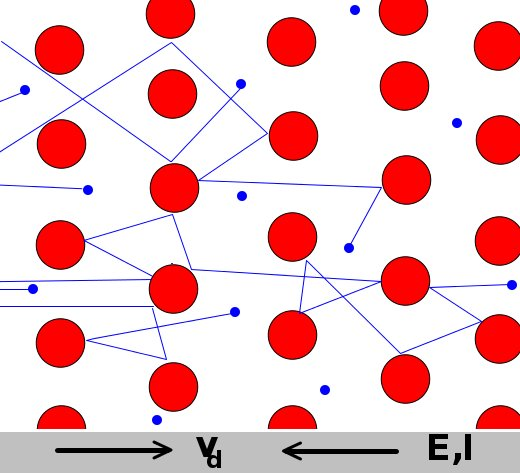
\includegraphics[scale=0.5]{Electrona_in_crystallo_fluentia.jpg}
  \end{center}
}

\frame[t] {
  \frametitle{Drude-Modell}

  \begin{tabular}{ll}
    Neigung: & $\vec E$ \\
    Kugel:   & Elektron \\
    Bumper:  & Ion
  \end{tabular}

  \vfill
  \hfill
  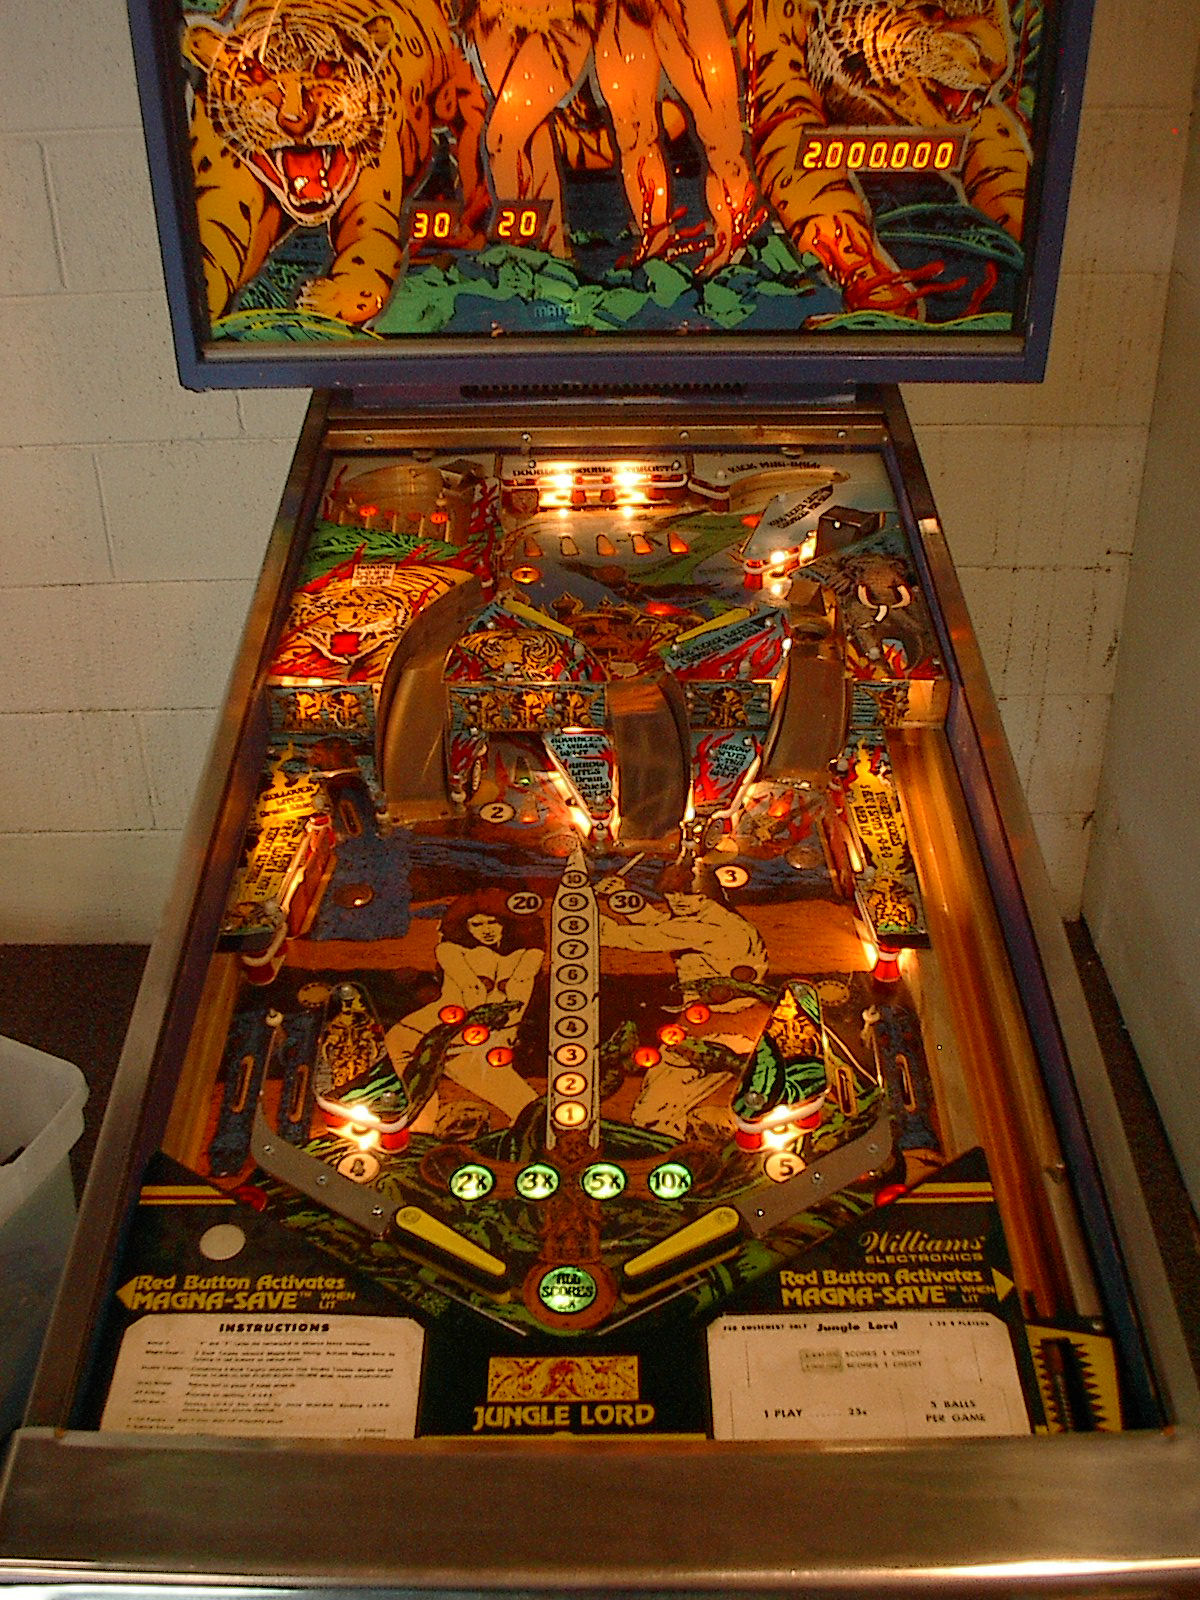
\includegraphics[scale=0.1]{flipper.jpg}
}

\frame[t] {
  \frametitle{Annahme freier Elektronen}

  Warum bewegen sich Elektronen zwischen Stößen frei?
  \begin{itemize}
    \item Valenzelektronen weitgehend delokalisiert und über den Kristall "`verschmiert"' (Leitungselektronen)
    \item Leitungselektronen sehen nicht "`nacktes"' Coloumb-Potential, sondern ein Pseudopotential
    \item kaum Elektron-Elektorn-Stöße wegen Pauli-Prinzip
    \item gute Näherung für Metalle mit einem Leitungselektron
  \end{itemize}

  \begin{center}
  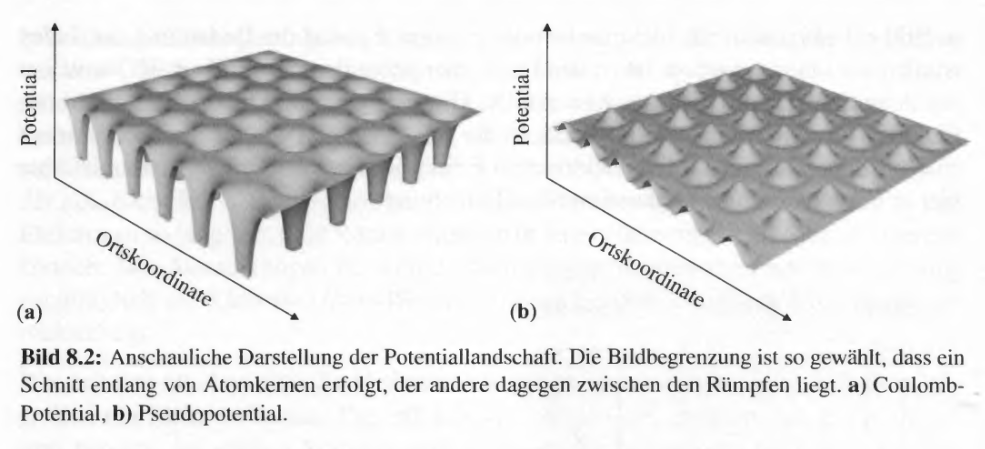
\includegraphics[scale=0.3]{potential.png}
  \end{center}
}

\subsection{Ohmsches Gesetz}
\frame[t] {
  \frametitle{Ohmsches Gesetz}

   \only<1>
   {
   \begin{itemize}
   \item Bewegungsgleichung für ein Elektron im Feld $\vec{E}$
     $$ \vec v(t) = \vec v_0 + \vec a  t = \vec v_0 + \frac{\vec F t}{m_\text{e}} = \vec v_0 + \frac{-\vec{\text{E}} \text{e} \cdot t}{m_\text{e}}$$

   \item mittlere freie Stoßzeit: $t = \tau$, $\vec v_0 = 0$
     $$ \vec v_\text{D} = \vec v(\tau) = - \frac{\text{e} \cdot \tau}{m_\text{e}} \vec{\text{E}} $$

   \item für die Stromdichte folgt
     $$ \vec{j} = -\text{e}n \vec v_\text{d} = \frac{n\text{e}^2\tau}{m_\text{e}}\vec{E} \ \ \Rightarrow \vec j \propto \vec E$$

   \item und damit für die Leitfähigkeit
     $$ \sigma = \frac{j}{E} = \frac{n\text{e}^2\tau}{m_\text{e}} $$
   \end{itemize}
   }

   \only<2>
   {
     \begin{itemize}
     \item $\sigma$ Tensor in anisotropen Materialien
     \item Ohmsches Gesetz zurückgeführt auf Elektronendichte $n$ und Stoßzeit $\tau$
     \item in der Herleitung werden \textit{alle} Leitungselektronen beschleunigt: Widerspruch zur Fermi-Dirac-Verteilung
     \item man erwartet große Anzahl von Stößen mit den Gitteratomen
     \item experimentell: freie Weglänge hängt von Temperatur und Qualität des Kristalls ab
     \item experimentell: freie Weglängen deutlich größer als vorhergesagt
     \end{itemize}
   }
}

\subsection{Probleme}
\frame[t] {
  \frametitle{Grenzen und Probleme des Drude-Modells}

  \begin{itemize}
    \item[\textcolor{green}{$\oplus$}] erklärt Ladungstransport in Metallen
    \item[\textcolor{green}{$\oplus$}] erklärt Hall-Effekt
    \item[\textcolor{green}{$\oplus$}] erklärt thermische Leitfähigkeit
    \item[\textcolor{green}{$\oplus$}] erklärt Wiedemann-Franz-Gesetz
    \\[1em]
    \item[\textcolor{red}{$\ominus$}] überschätzt elektronische Wärmekapazität von Metallen
    \item[\textcolor{red}{$\ominus$}] erklärt nicht, welche Materialien Leiter bzw. Isolatoren sind
    \item[\textcolor{red}{$\ominus$}] erklärt nicht Temperaturabhängigkeit der thermischen und elektrischen Leitfähigkeit
    \item[\textcolor{red}{$\ominus$}] viele Aussagen nur qualitativ richtig
  \end{itemize}

  \ \\[2em]

  Hauptproblem: beachtet nicht Pauli-Prinzip \only<2> { \\$\Rightarrow$ Quantenmechanik } 
}

\section{Quantenmechanisches Modell}
\subsection{Fermi-Energie}
\frame[t] {
  \frametitle{Teilchen im Kastenpotential (1D)}

  Teilchen in einem Potentialtopf der Länge $L$:
  $$ V(x,y,z) = 
    \left\{ 
      \begin{array}{rl}
        0 & 0 \le x \le L \\
        W & sonst
      \end{array}
    \right.
  $$

  \only<1>
  {
  \vfill
  \begin{center}
  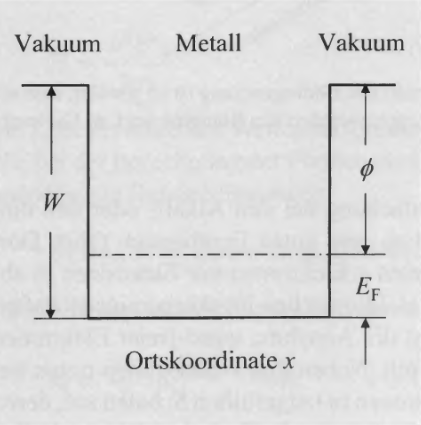
\includegraphics[scale=0.42]{kasten.png}
  \end{center}
  }

  \only<2>{
  stationäre Schrödingergleichung:
  $$ -\frac{\hbar^2}{2m}\Delta\psi(\vec r) + V(\vec r)\psi(\vec r) = E\psi(\vec r) $$
  }

  \only<3->{
  stationäre Schrödingergleichung im Metall:
  $$ -\frac{\hbar^2}{2\text{m}} \frac{\text{d}^2}{\text{d}x^2} \psi(x) = E\psi(x) $$
  }

  \only<4->{
    Lösung: ebene Wellen; Normierung $\psi_\text{n}(0) = \psi_\text{n}(\text{L}) = 0$
    $$ \psi_\text{n}(x) = \sqrt{\frac{2}{\text{L}}} \sin\left( \text{n} \frac{\pi}{\text{L}}x \right), \ \ k_\text{n} = \frac{\pi}{\text{L}}\text{n}$$
    $$ E_\text{n} = \frac{\hbar^2\pi^2}{2\text{m}\text{L}^2}\text{n}^2 $$
  }
}

\frame[t] {
  \frametitle{Teilchen im Kastenpotential (1D)}

  \begin{center}
  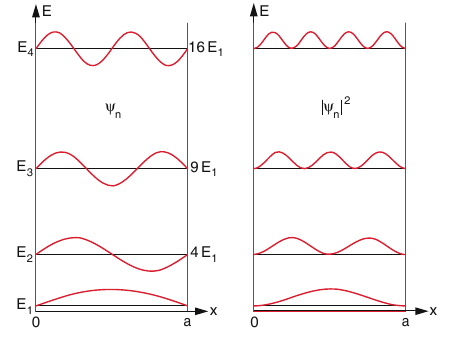
\includegraphics[scale=0.6]{teilchen.png} 
  \end{center}
}

\frame[t] {
  \frametitle{Teilchen im Kastenpotential (3D)}

  Teilchen in einem würfelförmigen Potential der Kantenlänge $L$:
  $$ V(x,y,z) = 
    \left\{ 
      \begin{array}{rl}
        0 & 0 \le x,y,z \le L \\
        W & sonst
      \end{array}
    \right.
  $$

  stationäre Schrödingergleichung im Metall:
  \only<1>
  {
  $$ -\frac{\hbar^2}{2\text{m}} \Delta \psi(\vec r) = E\psi(\vec r) $$
  }
  \only<2->
  {
  $$ -\frac{\hbar^2}{2\text{m}}\left( \frac{\text{d}^2}{\text{d}x^2} + \frac{\text{d}^2}{\text{d}y^2} +\frac{\text{d}^2}{\text{d}z^2} \right) \psi(\vec r) = E\psi(\vec r) $$
  }

  \only<3->
  {
  Lösung: $E = E_\text{x} + E_\text{y} + E_\text{z}$, $\psi(\vec r) = \psi_1(x) \psi_2(y) \psi_3(z)$
     $$ \psi(\vec r) = \text{C}\text{e}^{\text{i}\vec k \cdot \vec r},\ \ \ \boxed{E = \frac{\hbar^2k^2}{2m}} $$
     $$ k_i = \frac{2\pi}{L}n_i, \ \ \ \text{mit} \ i = (x,y,z) $$
  }
}


\frame[t] {
  \frametitle{Fermi-Energie}

  \only<1>
  {
  \vfill
  \begin{center}
  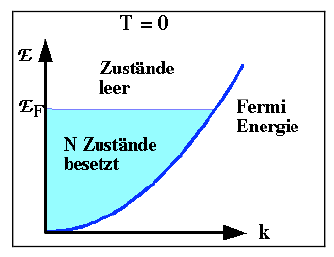
\includegraphics[scale=0.6]{fermienergie.png}
  \\
  Wie groß ist die Energie des höchstbesetzten Zustands (Fermi-Energie) bei Temperatur T=0K?
  \end{center}
  \vfill
  }

  \only<2->
  {
  \begin{itemize}
  \item N Elektronen besetzen die $\frac{\text{N}}{2}$ energetisch niedrigsten Zustände
  \item Seitenlänge der Einheitszelle im Impulsraum: $\frac{2\pi}{\text{L}}$
  \item besetzte Zustände füllen im Impulsraum eine Kugel mit Volumen $V = \frac{4}{3}\pi\text{k}_\text{F}^3$
  \item Anzahl der Zustände muss Anzahl der Elektronen N entsprechen
  $$ N = \frac{2 \cdot \text{Kugelvolumen}}{\text{Zustandsvolumen}} = 2\cdot \frac{\frac{4}{3}\pi\text{k}_\text{F}^3}{\left( \frac{2\pi}{\text{L}} \right)^3}$$
  \item für den Radius der Kugel folgt:
  $$ k_\text{F} = \left(\frac{3\pi^2\text{N}}{\text{V}} \right)^{\frac{1}{3}} \ \ \Rightarrow \text{E}_\text{F} = \frac{\hbar^2}{2\text{m}}\left( \frac{3\pi^2\text{N}}{\text{V}}\right)^{\frac{2}{3}}$$
  \end{itemize}
  }
}


\frame[t] {
  \frametitle{Fermi-Energie}

  Parametrisierung der Fermi-Energie über die Temperatur:
  $$ \text{k}_\text{B} \text{T}_\text{F} = \text{E}_\text{F} $$

  \begin{center}
  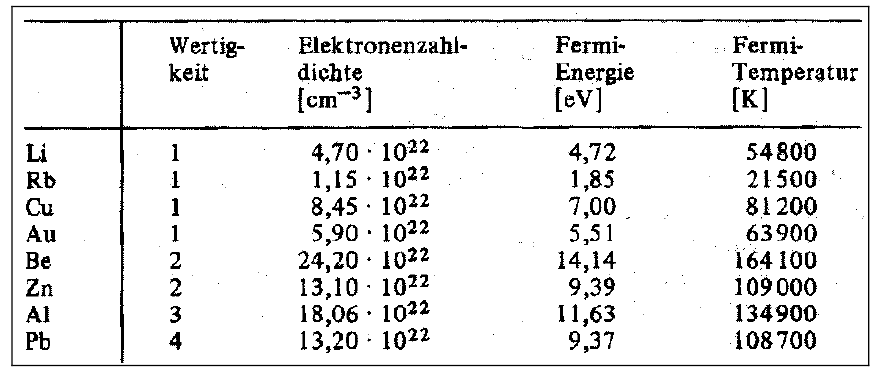
\includegraphics[scale=0.5]{fermitabelle.png}
  \end{center}

}


\frame[t] {
  \frametitle{Fermi-See}

  \begin{center}
  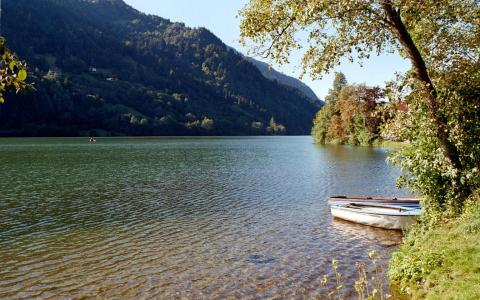
\includegraphics[scale=0.5]{see.jpg}
  \end{center}

}

\subsection{Zustandsdichte}
\frame[t] {
  \frametitle{Zustandsdichte}

  \begin{itemize}
  \item Anzahl der Zustände mit Wellenzahl kleiner k:
  $$ \text{N}(k) = \frac{\text{V} k^3}{3\pi^2} $$
  \item Anzahl der Zustände mit Energie kleiner E:
  $$ \text{N}(E) = \text{V} \frac{(2\text{m}E)^\frac{3}{2}}{3\pi^2\hbar^3} $$
  \item Zustandsdichte im Energieraum:
  $$ \frac{\text{dN}(E)}{\text{d}E} = \frac{\sqrt{2} V \text{m}^\frac{3}{2}}{\pi^2\hbar^3} \sqrt{E}$$
  \end{itemize}
}

\subsection{Fermi-Dirac-Verteilung}
\frame[t] {
  \frametitle{Fermi-Dirac-Verteilung}

  \only<1> {
  Besetzung für T $= 0$ klar: \\
  \begin{center}
  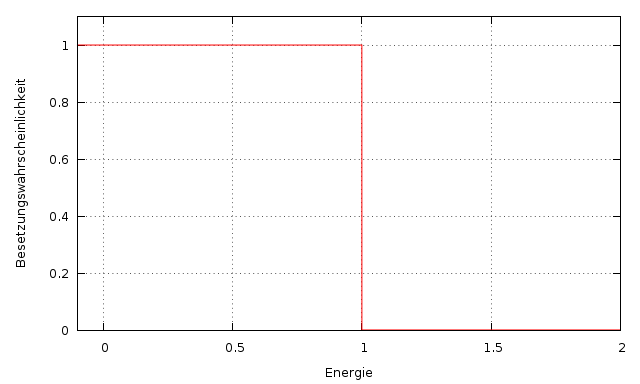
\includegraphics[scale=0.5]{fermidirac1.png}
  \\
  Und für $\text{T}>0$?
  \end{center}
  }

  \only<2>
  {
    \begin{itemize}
    \item Verteilung durch Fermi-Dirac-Verteilung gegeben:
    $$ \text{f}(E) = \dfrac{1}{\text{e}^{(E-\mu)/(\text{k}_\text{B}\text{T})} + 1} $$
    \item chemisches Potential $\mu = \left( \frac{\partial F}{\partial N}\right)_\text{T,V} $
    \item $E_\text{F} = \mu(\text{T}=0)$
    \item für T $<<$ $\text{T}_\text{F}$
    $$ \mu(\text{T}) \approx E_\text{F} \left[ 1 - \frac{\pi^2}{12} \left( \frac{\text{T}}{\text{T}_\text{F}} \right)^2\right] \approx E_\text{F}$$
    \item Aufweichung der Verteilung um Fermi-Kante von etwa $2\text{k}_\text{B}\text{T}$
    \end{itemize}
  }

  \only<3> {
  \begin{center}
  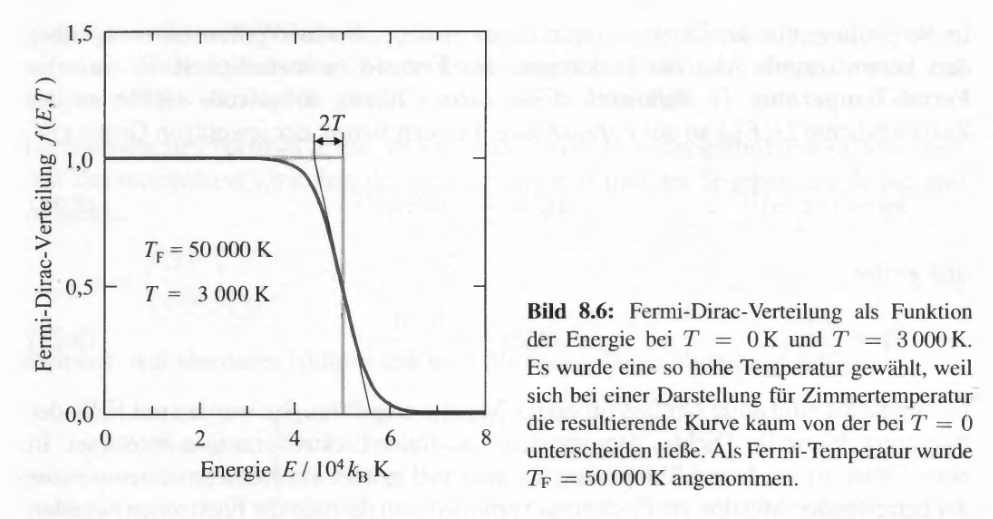
\includegraphics[scale=0.43]{fermidirac2.png}
  \end{center}
  }
}

\section{Voraussagen}
\subsection[spez. Wärme]{spezifische Wärme}
\frame[t] {
  \frametitle{spezifische Wärme des Elektronengases}

  \begin{itemize}
  \item innere Energie $u_0 = \frac{U}{V}$ des Fermi-Gases pro Volumen (T$=0$)
  $$ u_0  = \int_0^\infty E \cdot \text{D}(E) \cdot \text{f}(E, \text{T}) \text{d}E = \int_0^{\text{E}_\text{F}} E \cdot \text{D}(E)\text{d}E 
  = \frac{3\text{n}}{5} \text{E}_\text{F} = \frac{3\text{n}}{5} \text{k}_\text{B} \text{T}_\text{F}$$

  \only<1>
  {
  \item für die spezifische Wärme gilt:
  $$ \text{c}_\text{V}^\text{el} = \left( \frac{\partial u}{\partial T} \right)_\text{V} \ \ \text{mit } u(T) = \int_0^\infty E \cdot \text{D}(E) \cdot \text{f}(E, \text{T}) \text{d}E $$
  }

  \only<2>
  {
  \item für die spezifische Wärme gilt:
  $$ \text{c}_\text{V}^\text{el} = \left( \frac{\partial u}{\partial T} \right)_\text{V}; \ \ \delta u(T) = u(T) - u_0 \approx \text{n} \text{k}_\text{b} \text{T} \frac{T}{T_F}  - u_0$$
  }

  \only<3->
  {
  \item für die spezifische Wärme gilt:
  $$ \text{c}_\text{V}^\text{el} = \left( \frac{\partial u}{\partial T} \right)_\text{V} \approx \frac{2\text{n} \text{k}_\text{B} T}{\text{T}_\text{F}} $$

  \item spezifische Wärme pro Volumen eines Metalls 
  $$ \text{c}_\text{v}^\text{ges} = \gamma \text{T} + \left\{ 
    \begin{array}{lll}
    3n_A k_B & T > \theta   \ \\
    \beta T^3 & t << \theta
    \end{array} \right.
     $$
  }
  \end{itemize}
}


\frame[t] {
  \frametitle{spezifische Wärme des Elektronengases}

  \begin{center}
  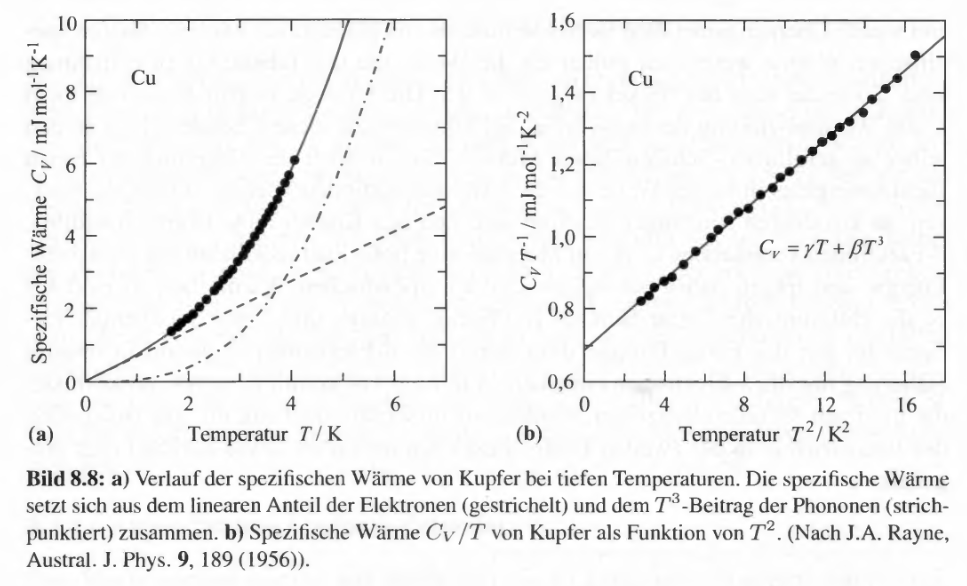
\includegraphics[scale=0.42]{spez.png}
  \end{center}
}

\frame[t] {
  \frametitle{effektive Masse}

  \begin{center}
  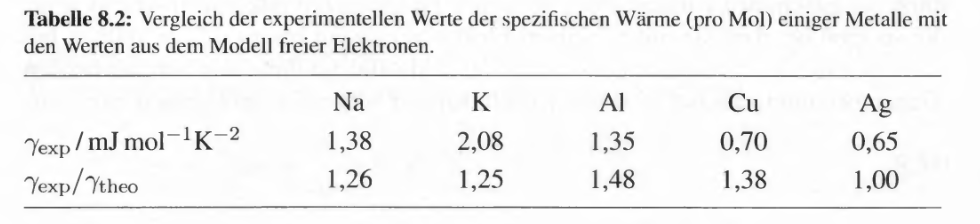
\includegraphics[scale=0.42]{exp.png}
  \end{center}


  \begin{itemize}
  \item Einführung einer effektiven Masse $\text{m}_\text{th}^*: \frac{\text{m}_\text{th}^*}{\text{m}} = \frac{\gamma_\text{exp}}{\gamma_\text{theo}}$
  \item hohe Werte für $\frac{\text{m}_\text{th}^*}{\text{m}}$ bei Übergangsmetallen: d-Wellenfunktionen mit Vorzugsrichtung
  \end{itemize}
}

\section{Quellen}
\frame {
  \frametitle{Quellen}

  \begin{itemize}
  \item Festkörperphysik, Hunklinger
  \item Solid State Physics, Ashcroft
  \item Wikipedia (Drude-Theorie, Elektronengas)
  \end{itemize}
}


% effektive massen?

%\subsection{Leitfähigkeit}
%\frame[t] {
%  \frametitle{elektrische Leitfähigkeit}
%
%}
%
%\subsection{Wärmeleitung}
%\frame[t] {
%  \frametitle{Wärmeleitung}
%
%  \begin{itemize}
%  \item Wärmeleitung: $\vec{j_Q} = K \nabla T$
%  \item $c_\text{el} = \frac{\pi^2}{2} k_B n  \frac{T}{T_F}$
%  \item $K = \frac{1}{3} \frac{\pi^2}{2} k_B n \frac{T}{T_F} v_F v_F \tau$
%  \item $v_F^2 = 2 \frac{E_F}{m} = \frac{2 k_b T_F}{m}$
%  \item $K = \frac{\pi^2}{3} \frac{k_B^2 n T \tau}{m}$
%
%  \end{itemize}
%
%}
%
%\subsection{Wiedemann-Franz-Gesetz}
%\frame[t] {
%  \frametitle{Wiedemann-Franz-Gesetz}
%
%}
%
%\subsection{Elektronenstreuung}
%\frame[t] {
%  \frametitle{Elektronenstreuung}
%
%  \only<1>
%  {
%  Streuung an Defekten
%  \begin{itemize}
%  \item Wechselwirkung mit Gitterstörungen
%  \item elastische Streuung: Richtung des Wellenvektors ändert sich, Betrag bleibt konstant: $$ \vec{\text{k}} = \vec{\text{k'}} + \vec{\text{K}} $$
%  \item Impulsübertrag $\hbar \text{K}$ wird vom Gitter übernommen, $\text{K} \le 2\text{k}$
%  \end{itemize}
%
%  \begin{center}
%  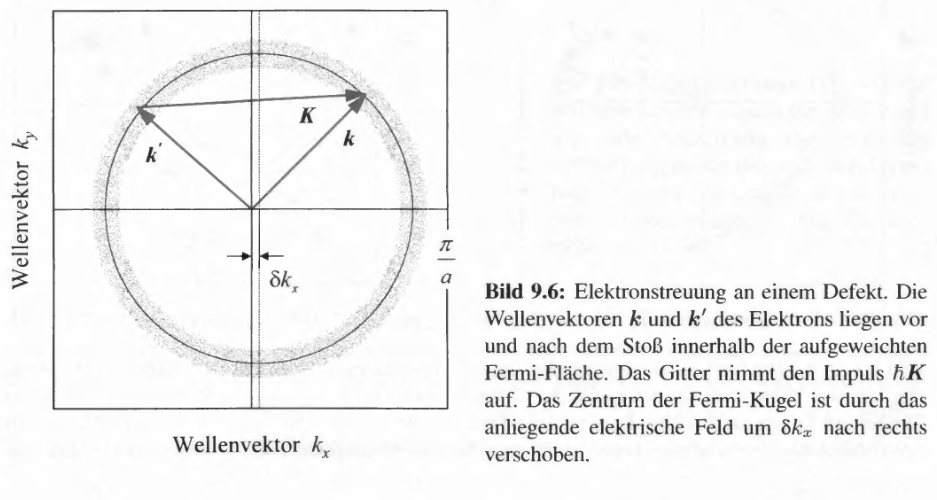
\includegraphics[scale=0.3]{defektstreuung.png}
%  \end{center}
%  }
%
%  \only<2>
%  {
%    Streuung an Phononen
%    \begin{itemize}
%    \item inelastische Streuung 
%    \item $\vec{\text{k}} = \vec{\text{k'}} \pm \vec{\text{q}} + \vec{\text{G}}$
%    \item da $\text{E}_\text{F} >> \hbar\omega_\text{D}$, gilt: $\text{k} \approx \text{k'}$
%    \end{itemize}
%  }
%}


\end{document}
